\documentclass[xcolor=pdftex,dvipsnames,table]{beamer}
\usepackage{beamerthemesplit}
\usepackage{minted}
\usepackage{hyperref}
\usepackage{textcomp}
\usetheme{Madrid}
\usecolortheme{crane}
\title{An Alternative Introduction to Programming}
\subtitle{Read: A Tutorial of the Scheme Programming language}
\author{Shen Zheyu}
\date{\today}
\begin{document}
\maketitle
\begin{frame}[allowframebreaks]
  \frametitle{Table of Contents}
  \tableofcontents
\end{frame}
\begin{frame}
  \frametitle{Introduction}
  \begin{itemize}
    \item Shen Zheyu, sophomore ECE student
    \item My GitHub: \url{http://github.com/arsdragonfly/}
    \item SSTIA projects \url{https://github.com/SSTIA}
    %\vspace{1.3in}
  \end{itemize}
  \begin{columns}
    \begin{column}{0.5\textwidth}
      \begin{center}
        \begin{figure}
          
\includegraphics[width=0.6\textwidth]{avatar}
        \end{figure}
      \end{center}
    \end{column}
    \begin{column}{0.5\textwidth}
      \vspace*{\fill}
      \begin{center}
        \begin{figure}
          
\includegraphics[width=0.6\textwidth]{SSTIA}
        \end{figure}
      \end{center}
    \end{column}
  \end{columns}
\end{frame}
\begin{frame}[fragile]
  \frametitle{Overview}
  This seminar is intended to provide a different introduction to programming from VG101 (and arguably many other courses).
  In a (hopefully) friendly way, you'll learn many useful things unlikely to be found in other introductory material.
  \pause

  Much of the content is adapted from \textcolor{Blue}{\textit{The Little Schemer, Fourth Edition}} by D. P. Friedman and M. Felleisen.
  If you're very interested, You may also want to read \textcolor{Blue}{\textit{Structure and Interpretation of Computer Programs}} by H. Abelson and G. J. Sussman.
  \begin{center}
    \begin{figure}
      
\includegraphics[width=0.4\textwidth]{SICP.png}
    \end{figure}
  \end{center}
\end{frame}
\begin{frame}
  \frametitle{Setup}
  To begin with this seminar, you need to have a Scheme interpreter up and running.
  I personally recommend \textcolor{Blue}{Racket (\url{www.racket-lang.org})}, though other programs may also work (MIT Scheme, Guile, Chez Scheme, etc.).
\end{frame}
\begin{frame}[fragile]
  \frametitle{Setup}
  Before we start, we need to make sure that every program contains the following definitions of primitive functions:
  \begin{minted}{scheme}
    (define add1
      (lambda (n)
        (+ n 1)))
    (define sub1
      (lambda (n)
        (- n 1)))
  \end{minted}
  It's recommended for this seminar now that you write your program in a single source code file, so that latter definitions of functions can build upon previous already-written ones.
\end{frame}
\begin{frame}
  \frametitle{Setup}
  \begin{center}
    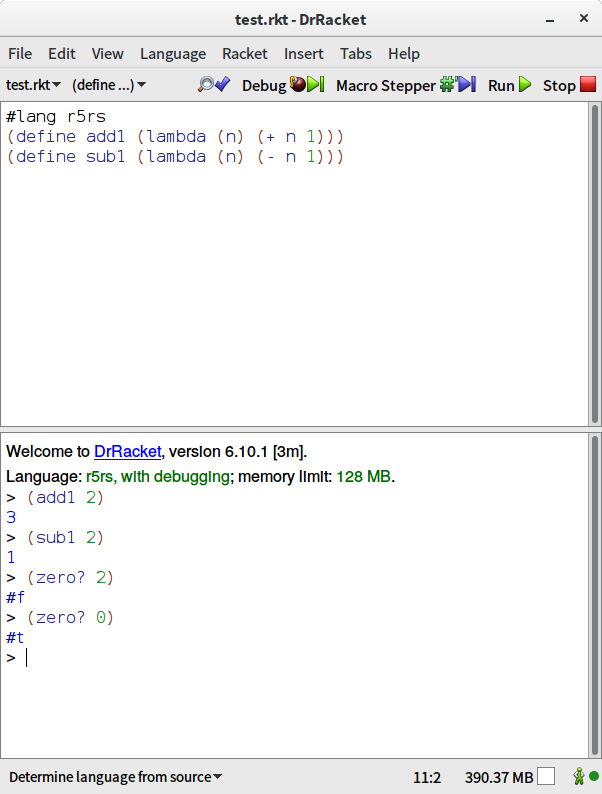
\includegraphics[height=0.8\textheight]{screenshot}
  \end{center}
\end{frame}

\section{Numbers}

\begin{frame}[fragile]
  \frametitle{Arithmetic on Natural Numbers}
    \begin{itemize}
      \item What's the answer of \mintinline{scheme}{(add1 0)}?
      \item \emph{1}.
      \pause
      \item What's the answer of \mintinline{scheme}{(sub1 3)}?
      \item \emph{2}.
      \pause
      \item What's the answer of \mintinline{scheme}{(add1 (add1 0))}?
      \item \emph{It's the answer of \mintinline{scheme}{(add1 1)}.}
      \pause
      \item What's the answer of \mintinline{scheme}{(add1 1)} then?
      \item \emph{2}.
    \end{itemize}
\end{frame}

\begin{frame}[fragile]
  \frametitle{Arithmetic on Natural Numbers}
    \begin{itemize}
      \item What's the answer of \mintinline{scheme}{(zero? 0)}?
      \item \mintinline{scheme}{#t}\emph{, which means "true".}
      \pause
      \item What's the answer of \mintinline{scheme}{(zero? 810)}?
      \item \mintinline{scheme}{#f}\emph{, which means "false".}
      \pause
      \item What's the answer of \mintinline{scheme}{(zero? (sub1 (sub1 2)))}?
      \item \mintinline{scheme}{#t}
    \end{itemize}
\end{frame}

\begin{frame}[fragile]
  \frametitle{$\lambda$ ?}
    \begin{itemize}
      \item What's the answer of \mintinline{scheme}{(lambda (x) (add1 (add1 x)))}?
      \item \emph{A \textrm{lambda expression}, which is similar to a mathematical function.}
      \pause
      \item What's the answer of \\
      \mint{scheme}{(define add2 (lambda (x) (add1 (add1 x))))}
      \mint{scheme}{(add2 (add1 3))}
      ?
      \item \emph{6.}
    \end{itemize}
\end{frame}

\begin{frame}[fragile]
  \frametitle{$\lambda$ ?}
    \begin{itemize}
      \item How does \mintinline{scheme}{(add2 (add1 3))} work?
      \item \emph{We first ask the question: what is \mintinline{scheme}{(add1 3)}?}
      \pause
      \item What is the answer of \mintinline{scheme}{(add1 3)}?
      \item \emph{4.}
      \pause
      \item What's the answer of \mintinline{scheme}{(add2 4)} then?
      \item \emph{It becomes \mintinline{scheme}{((lambda (x) (add1 (add1 x))) 4)}.}
      \pause
      \item Then?
      \item \emph{We substitute \textrm{x} for \textrm{4} in the \textrm{lambda expression}.}
      \pause
      \item What will we get then?
      \item \emph{\mintinline{scheme}{(add1 (add1 4))}}
      \pause
      \item Is that how we get 6?
      \item \emph{Yes.}
    \end{itemize}
\end{frame}

\begin{frame}[fragile]
  \frametitle{\mintinline{scheme}{cond?}}
  \begin{itemize}
    \item How does the following definition work out?
    \begin{minted}{scheme}
      (define one?
        (lambda (x)
          (cond
            ((zero? (sub1 x)) #t)
            (else #f))))
    \end{minted}
    \item \emph{We'll figure it out soon\texttrademark.}
    \pause
    \item What's the answer of \mintinline{scheme}{(one? 1)}?
    \item \mintinline{scheme}{#t}.
    \pause
    \item What's the answer of \mintinline{scheme}{(one? 2)}?
    \item \mintinline{scheme}{#f}.
  \end{itemize}
\end{frame}

\begin{frame}[fragile]
  \frametitle{\mintinline{scheme}{cond?}}
    \begin{minted}{scheme}
      (define one?
        (lambda (x)
          (cond
            ((zero? (sub1 x)) #t)
            (else #f))))
    \end{minted}
  \begin{itemize}
    \item How does the above definition work out?
  \end{itemize}
\end{frame}

\end{document}
